\documentclass[a4paper,12pt]{article}

\author{Bromberry games}
\title{Zvery Rules}
\setlength{\parindent}{0mm}
\usepackage{graphicx}

\begin{document}
\maketitle

\section{Overview}
Zvery is a game about fighting and catching creatures.
Your goal is to create or find the strongest creatures in the world of Plasoder and then destroy your opponent with them.
\section{Components}
Zvery has 3 different types of cards.
Creatures, abilities and mutations.
\subsection{Creatures}
\begin{center}
	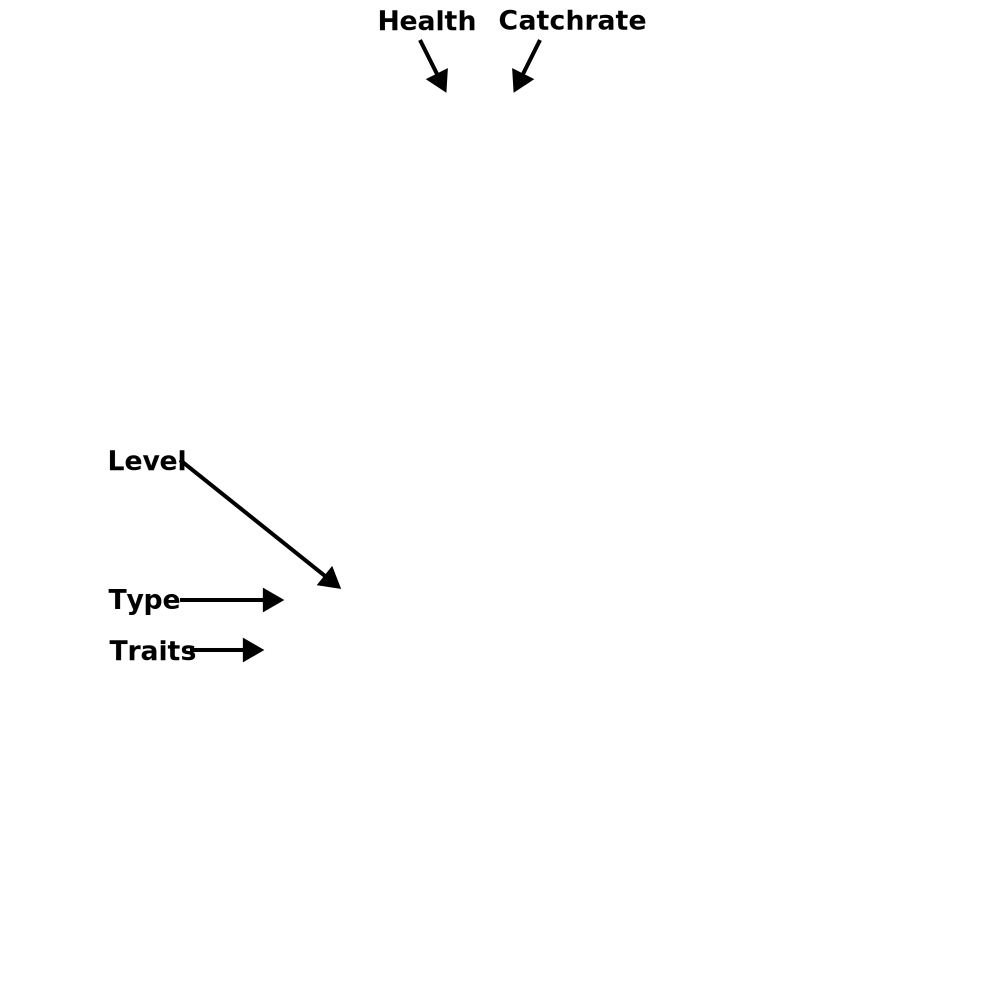
\includegraphics[scale=0.45]{./media/creature_explained}
\end{center}
A creature has the following characteristics.
\subsubsection{Level}
Describes the strength of a creature. Generally, the higher the level of the creature, the tougher it will be to battle or catch.
\subsubsection{Type}
There are 5 different types a creature can have:
\textbf{Radioactive, Bubblegum, Plasma, Void} and \textbf{Crystal}.
The Type of a creature gives an indication of how it will behave in 
battle and will determine what \textbf{Abilities} it can use.
\subsubsection{Health}
The amount of Health the creature has. Important for combat.
\subsubsection{Catchrate}
The higher the number, the tougher it will be to catch the creature.
Refer to the section on catching a creature.
\subsubsection{Traits}
Traits are effects unique to the creature that give it extra effects in combat. 
\subsection{Abilities}
Abilities also come in five types, and it must be of the same type as the creature.  
An ability has 4 skills.
Every skill has an activation cost which you need to fulfill so you can use the effect of the skill.
Skills allow your creature to damage an opposing creature, heal your own creatures or manipulate the battle in other ways. 
\subsubsection{Activation costs}
\paragraph{Exact value}
Indicated by a dice value. Requires the exact dice value
\paragraph{Powerup}
Indicated by a number. Needs the sum of dice values used on this to be equal or higher than the number
\paragraph{X}
Needs any dice used.
\paragraph{Same}
Needs the same value of dice used for every equal sign.
\paragraph{Chain}
Requires consecutive dice values used.


\subsection{Mutations}
The world around you is constantly changing and evolving at a rapid pace.
So your creatures mutate after every battle.
Once your creature mutated it cannot mutate back.
Mutation cards also have 5 different types, but these do NOT have to be the same as the creature's type.
Any mutation card can go on any creature.
Mutation cards come in 2 different variants.
\subsubsection{Upgrades}
Modify how a creature behaves. Place these over your creature.
\subsubsection{Abilities}
An ability which can be used by any creature. Place these beneath your creatures abilities.

\section{Game structure}
Start by shuffling the mutation deck and the ability deck.
Separate the creatures into 3 decks according to their levels. All level 1 creatures into 1 deck, level 2 into another etc. Then shuffle each of the creature decks and place them face down.
Give each player 5 d6. Then determine who starts the game. 
Place 3 level 2 creatures face up. The starting player now chooses one of the 3 creatures as his starter. Then the other player chooses a creature.
After that, each player looks through the ability deck and takes the first ability that matches their creature's type and places it beneath their creature.
Now take 3 level 1 creatures and place them face up on the field. Finally, place 3 mutation cards face up on the field.
You are ready to start the game!

\subsection{The Phases}
\begin{enumerate}
	\item Player chooses one or two creatures to battle
	\item Battle
	\item Distribute mutations 
	\item Refill creature cards
	\item Refill mutations
	\item Switch player
\end{enumerate}

\subsubsection{Choose creatures to battle}
The player picked their starter last starts the first battle. They may choose up to 2 creatures to fight, and the other player gets to control them in battle.
Now, place a d20 on every creature and set it to their health value. The current player now chooses as many open mutations as the combined level of creatures he fights (max. 3). Place the selected mutations in the middle of the battlefield. 
Now move on to the Battle phase.
\subsubsection{Battle}
A battle is comprised of 1 or more turns with each turn running through the following steps.
\begin{enumerate}
	\item Before roll
	\item Only in wild battles: Choose catch or combat
	\item Only in wild battles: Catch
	\item Creatures die
	\item Roll for combat
	\item After roll
	\item Combat
	\item End of turn
\end{enumerate}
\subsubsection{Before roll}
Before roll effects from cards activate.
\subsubsection{Choose catch or combat}
Every turn, the currently active player has to decide whether he wants to catch the wild creature or fight it.
\subsubsection{Catch}
This step only activates when the current player chose catch.
They then declare which creature they want to catch and roll 5 d6, no more and no less.
If the total sum of eye numbers is greater than or equal the creatures 
catchrate + current health they succeed in catching.
If it is lower, they may choose to leave any of their rolled dice on the creature and try to catch the creature again next turn with their remaining dice.
If they do not want to catch the creature next turn, they can then take back their dice from the creature and battle normally with them.
If they tried to catch a creature this turn then they cannot roll dice for combat this turn. 
\subsubsection{Creatures die}
Any creature whose health is below 0 now gets removed from the battlefield. Turn the dead creatures face down. 
\subsubsection{Roll for combat}
Both players roll 5 d6 unless specified otherwise by a card.
\subsubsection{After roll}
After roll effects activate.
\subsubsection{combat}
The controlling player starts by activating one or more \textbf{skills}. Then passes to the wild player. The wild player then activates abilities and passes back.
If a player at one point does not use a skill, they are out of this turn and will not be able to activate a skill later this turn. Once both players have activated no \textbf{skills} the turn ends. The player who has more unused dice starts the next turn.
Once a creature has 0 or less health, it is \textbf{bleeding out} and will die the next turn. If you manage to heal it above 0 during this turn, it can keep fighting.
\\
\subsubsection{End of turn}
End of turn effects activate. Then the phases start from the beginning again until one player has no creature that can battle any longer. When that happens move on to distribute mutations and move all dead wild creatures and their abilities into the discard pile.
\\
\subsection{Distribute mutations}
After every battle players receive mutations according to their performance in battle.
If the current player did neither catch nor kill a creature they will receive 1 mutation.\\
The wild player may select 1 mutation for every creature the current player caught and 1 mutation for every creature they killed. \\
The current player can select
\begin{itemize}
	\item 1 mutations for every level 1 creature you killed
	\item 2 mutations for every level 2 creature you killed
	\item 3 mutations for every level 3 creature you killed
\end{itemize}
Players alternate, starting with the current player, choosing among the mutations the current player selected before battle. 
If at some point this all selected mutations cards are gone, players draw the rest from the top of the mutation pile.\\
Now both players have to put the mutation cards immediately on their creatures or throw them on the discard pile.
\subsection{Refill creature cards}
For every creature that was battled this turn, draw a new one with a level +1 than the one before. Place it open on the battlefield.
\subsection{Refill mutations}
Draw new mutations and place them open on the battlefield so that 3 mutations are face up again.
\subsection{Switch player}
Now the current player becomes the wild player and the other way around.
Move back to step 1.
\subsection{End of game}
Once a level 3 creature has either been killed or caught the game moves into its final phase. One epic battle between both players.
The winner of that battle wins the game.
\section{Glossary}
\textbf{stun X}: Put a stun card with value X on the creature that is being stunned.
A creature that is stunned cannot use abilities but may use traits.
Stun can be removed during a players turn by removing dice from their roll that sum up to the value of the stun or higher. 
\\

\textbf{shatter X}: Choose X of your rolled unused dice. If a chosen dice is even, gain 2 new unused dice with value halve of the chosen dice. 
If a chosen dice is odd gain 2 new dice one with halve the value of the chosen dice round down the other with halve the value round up.
\\
\\
\textbf{fuse X}: Do X times. Choose 2 of your rolled dice. Add up their value and gain a new unused dice with that value. If the sum is above 6, subtract 6 from the sum and gain a new dice with the resulting value. For example, when fusing a 4 and 5, the sum is 9. Subtracting 6, you would gain a die with value 3.
\\
\\
\textbf{set X}:
Set the value of X of your used or unused dice to whatever value you want.
\\
\\
\textbf{increment X}:
Do X times: Increment any of your dice by 1.
\\
\\
\textbf{decrement X}:
Do X times: Decrement any of your dice by 1.
\\
\\
\textbf{strength X}:
A creature deals +X damage with every attack.
\\
\\
\textbf{fortitude X}:
A creature receives -X damage with every attack.
\end{document}

